% ****** Start of file apssamp.tex ******
%
%   This file is part of the APS files in the REVTeX 4.1 distribution.
%   Version 4.1r of REVTeX, August 2010
%
%   Copyright (c) 2009, 2010 The American Physical Society.
%
%   See the REVTeX 4 README file for restrictions and more information.
%
% TeX'ing this file requires that you have AMS-LaTeX 2.0 installed
% as well as the rest of the prerequisites for REVTeX 4.1
%
% See the REVTeX 4 README file
% It also requires running BibTeX. The commands are as follows:
%
%  1)  latex apssamp.tex
%  2)  bibtex apssamp
%  3)  latex apssamp.tex
%  4)  latex apssamp.tex
%
\documentclass[%
 reprint,
%superscriptaddress,
%groupedaddress,
%unsortedaddress,
%runinaddress,
%frontmatterverbose, 
%preprint,
%showpacs,preprintnumbers,
%nofootinbib,
%nobibnotes,
%bibnotes,
 amsmath,amssymb,
 aps,
%pra,
%prb,
%rmp,
%prstab,
%prstper,
%floatfix,
]{revtex4-1}

\usepackage{graphicx}% Include figure files
\usepackage[utf8]{inputenc}
\usepackage{dcolumn}% Align table columns on decimal point
\usepackage{bm}% bold math
%\usepackage{hyperref}% add hypertext capabilities
%\usepackage[mathlines]{lineno}% Enable numbering of text and display math
%\linenumbers\relax % Commence numbering lines

%\usepackage[showframe,%Uncomment any one of the following lines to test 
%%scale=0.7, marginratio={1:1, 2:3}, ignoreall,% default settings
%%text={7in,10in},centering,
%%margin=1.5in,
%%total={6.5in,8.75in}, top=1.2in, left=0.9in, includefoot,
%%height=10in,a5paper,hmargin={3cm,0.8in},
%]{geometry}

\begin{document}

\preprint{APS/123-QED}

\title{Espectros Atómicos}% Force line breaks with \\
\thanks{}%

\author{Jesus Prada}
 \email{jd.prada1760@uniandes.edu.co}
 \altaffiliation[Also at ]{Departamento de Física, Universidad de los Andes}%Lines break automatically or can be forced with \\
\author{Sergio Iv\'an Rey}%
 \email{si.rey1826@uniandes.edu.co}
\affiliation{%
 Departamento de Física, Universidad de los Andes
}%

\date{13/8/2015}% It is always \today, today,
             %  but any date may be explicitly specified

\begin{abstract}

\end{abstract}


\keywords{}%Use showkeys class option if keyword
                              %display desired
\maketitle

%\tableofcontents

\section{\label{sec:level1}Introducci\'on}

\begin{equation}
V(t) = V_0 e^{\frac{-\gamma t}{2}}\cos(\omega_a t + \delta)
\label{eq:amortiguado}
\end{equation}

\section{\label{sec:level1}Montaje experimental}

\section{\label{sec:level1}Resultados y An\'alisis}
\subsection{\label{sec:level2}Calibración con He}
Debido a que no conocíamos en principio la relación de la medida de la regla proporcionada, y tampoco conocíamos las unidades de dicha regla, necesitabamos de unas líneas espectrales de referencia para poder calibra el montaje. En nuestro caso, dado que queríamos estudiar las líneas del hidrógeno y la constante de Rydberg, usamos helio para dicho calibre. El helio tiene cuatro líneas espectrales fuertes en el espectro visible, por lo cual resulta un buén candidato de referencia. Los valores teóricos de longitud de onda de las líneas observadas de Helio junto a sus respectivas distancias observadas en la regla, se encuentran consignadas en la tabla \ref{table:helio}.

\begin{table}[h!]
\centering
 \begin{tabular}{|c|c|} 
 \hline
 $Regla (\pm0.2)$ & $Longitud de onda (nm)$ \\ [0.5ex] 
 \hline\hline
5.2 &		447.18\\
8.6 &		501.57\\
12.1 &		587.56\\
14.0 &		667.82\\
[1ex] 
 \hline
 \end{tabular}
 \caption{Espectro del helio para el calibre de la regla.}
 \label{table:helio}
\end{table}

En este caso, no conocíamos las unidades de la regla, por lo que las distancias medidas las tomamos adimensionales. En principio pensábamos que la relación entre la medida observada en la regla era lineal, sin embargo, si se procedía a hacer cálculos con este supuesto, se obtenían errores relativamente grandes para algunas longitudes de onda mas que otras. Por esto, pensamos que la relación de calibración no era necesariamente lineal. De esta manera, la siguiente relación más simple que se nos ocurría, teniendo en cuenta que el manejo de distancias y perspectiva es cuadrático, era una parábola. Al final descubrimos que dicha relación cuadrática se ajustaba muy bien a las líneas del helio. En la figura \ref{fig:calibre} se puede apreciar una gráfica de la longitud de onda de las líneas del helio contra la distancia medida. En esta misma figura graficamos el mejor ajuste primero suponiendo que la relación era lineal y luego suponiendo que era cuadrática; claramente el mejor ajuste, que pasa por todos los puntos según el error de resolución es el cuadrático.\\

\begin{figure}[h]
\caption{Curva de calibración con las líneas espectrales del Helio}
\centering
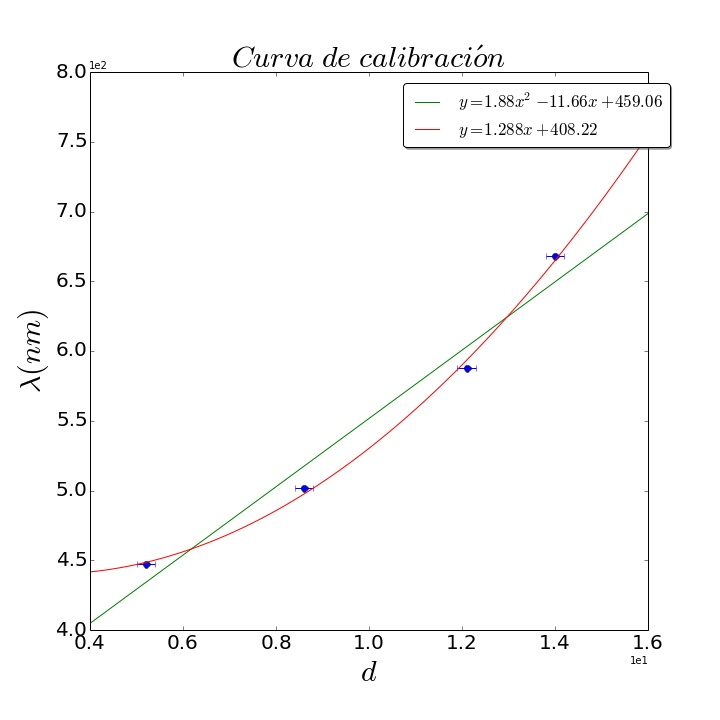
\includegraphics[width=0.45\textwidth]{calibre}
\label{fig:calibre}
\end{figure}

Con el ajuste cuadrático y los datos proporcionados podemos estimar el error asociado a cada parámetro de la parábola teniendo en cuenta la variación de la "lokelihood", una medida de qué tan cercano es el ajuste a los datos experimentales. Estos errores vienen casi dados por la rutina de optimización de Scipy. Una vez obtenidos estos errores se puede hacer la conocida propagación de error para calcular el error de longitud de onda asociado a cada medida de distancia que se introduzca en el ajuste.\\

\subsection{\label{sec:level2}Constante de Rydberg}
Una vez calibrado el instrumento, podemos proceder a analizar los datos de diferentes espectros de distintos átomos, diferentes del helio claramente. En este caso, analizaremos las líneas espectrales del hidrógeno y su relación con las series de Balmer para encontrar la constante de Rydberg de acuerdo a la ecuación \ref{eq:balmer}.\\

En la tabla \ref{table:hidrogeno} se encuentran consignados los datos teóricos y experimentales con los respectivos errores para las líneas espectrales del hidrógeno. Aquí también consignamos el la transición de niveles energéticos que provocan cada línea.\\

\begin{table}[h!]
\centering
 \begin{tabular}{|c|c|c|c|c|} 
 \hline
 $Regla (\pm0.2) $ & $\lambda_{Exp} (nm)$ & $\lambda_{Teo} (nm)$ & $\epsilon$ & $ n \rightarrow 2 $\\ [0.5ex] 
 \hline\hline
3.8 &	441.01 $\pm$ 8.9 & 434.057 & 1.6\% & 5\\
7.4 &	475.15 $\pm$ 9.9 & 486.135 & 2.3\% & 4\\
13.5 &	664.72 $\pm$ 16.0& 656.279 & 1.8\% & 3\\
[1ex] 
 \hline
 \end{tabular}
 \caption{Líneas espectrales del hidrógeno con sus niveles de transición n.}
 \label{table:hidrogeno}
\end{table}

De esta tabla cabe resaltar que las líneas teóricas caen en el rango de error de las experimentales y que los errores son razonables. Estos errores, como ya se había mencionado corresponden a la propagación de error de la resolución de la regla. Si uno mira con atención el error absoluto asociado a cada medición es del mismo orden de magnitud que el error de resolución, esto es, $0.2/d$, donde $d$ es la conocida medida en la regla. Existen además otras fuentes de error como el índice de refracción del aire, el cual puede variar un poco la longitud de onda observada respecto a la del vacío, sin embargo, este error es muy pequeño. Se puede afirmar que el índice de refracción del aire es $1$ cometiendo un error del orden de $0.1\%$.\\

Si graficamos ahora los valores de $frac{1}{\lambda_{Exp}}$ y $\frac{1}{n^2}$, encontraríamos, gracias a la ecuación \ref{eq:balmer} que la pendiente sería la constante de Rydberg. En la figura \ref{fig:balmer} se pueden apreciar los datos de la tabla \ref{table:hidrogeno} graficados con su respectivo ajuste lineal.\\

\begin{figure}[h]
\caption{Serie de Balmer del Hidrógeno}
\centering
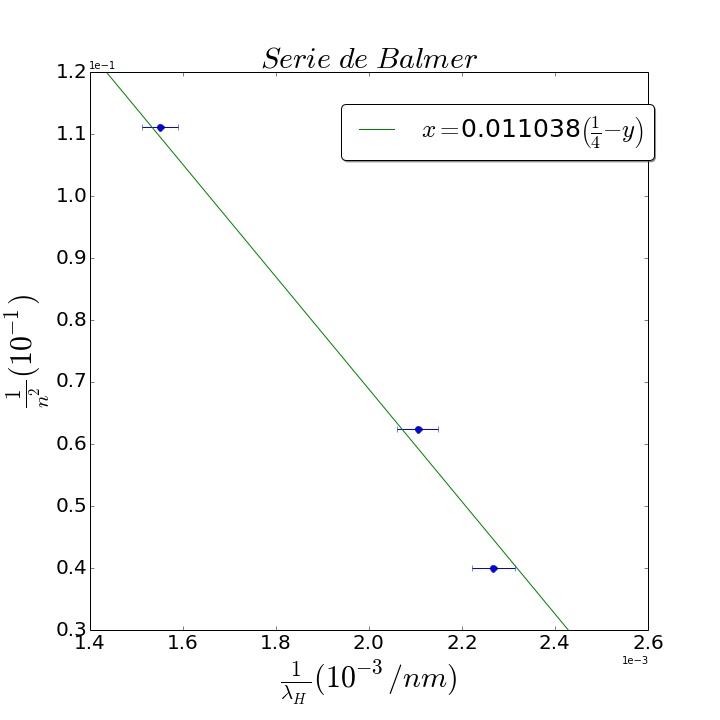
\includegraphics[width=0.45\textwidth]{balmer}
\label{fig:balmer}
\end{figure}

En este caso obtuvimos un valor de la constante de Rydberg dado por $R_{Exp} = 0.011038 \pm 0.00014\ nm^{-1}$. Este error fue calculado con el parámetro de error dado por el ajuste, el cual tiene encuenta también el error asociado a la longitud de onda. El valor teórico, el cual es de $R_{Teo} = 0.01097373 nm^{-1}$ entra en el rango del error proporcionado y determina un error de $0.6\%$, lo cual es bastante bajo debido a que se hizo un análisis lineal sobre varios datos, lo cual reduce el error en proporción al número de datos que se tengan (si son datos acordes al ajuste).\\


\subsection{\label{sec:level2}Otros espectros atómicos}
Una vez calculada la constante de Rydberg se procedió a estudiar los espectros de gases de mercurio, argón y kriptón. Debido a que estos gases son de átomos mucho más pesados, las soluciones de onda para los electrones son en este caso más complejas que la del hidrógeno, dado que en estos casos, los electrones que provocan las líneas espectrales pueden ser influenciados por la nube electrónica formada por los demás electrones. Por esto, las series de estos átomos pueden no ser descritas por una ecuación simple como la ecuación \ref{eq:balmer}. En este sentido, en esta sección nos limitamos a calcular el valor experimental de longitud de onda de cada una de las líneas observadas y compararlas con sus respectivos valores teóricos. Estos datos experimentales y teóricos se encuentran en la tabla \ref{table:otros}.\\


\begin{table}[h!]
\centering
 \begin{tabular}{|c|c|c|c|c|} 
 \hline
 $Atomo$ & $Regla (\pm0.2) $ & $\lambda_{Exp} (nm)$ & $\lambda_{Teo} (nm)$ & $\epsilon$\\ [0.5ex] 
 \hline\hline
 Hg & 4.1  &	441.99 $\pm$ 9.0  & 435.83 & 1.4\% \\
 Hg & 10.5 &	543.77 $\pm$ 12.2 & 546.07 & 0.42\% \\
 Hg & 11.7 &	580.07 $\pm$ 13.5 & 579.06 & 0.17\% \\
 \hline
 Ar & 5.1  &447.70 $\pm$ 9.1  & 451.07 & 0.75\% \\
 Ar & 7.3  &473.54 $\pm$ 9.9  & 476.48 & 0.61\% \\
 Ar & 14.2 &673.17 $\pm$ 17.2 & 671.85 & 0.20\% \\
 Ar & 14.4 &	681.64 $\pm$ 17.5 & 696.54 & 2.14\% \\
 \hline
 Kr & 10.8 &	 552.34  $\pm$ 12.5 & 557.02 & 0.84\% \\
 Kr & 11.8 &	 583.34  $\pm$ 13.7 & 587.09 & 0.64\% \\
 Kr & 13.5 &	 644.73  $\pm$ 16.0 & 642.01 & 0.42\% \\
[1ex] 
 \hline
 \end{tabular}
 \caption{Líneas espectrales del hidrógeno con sus niveles de transición n.}
 \label{table:otros}
\end{table}

De esta tabla es importante notar que la mayoría de las líneas calculadas tienen longitudes de onda teórica que entran dentro del rango de error calculado. También es importante notar que el error calculado con propagación de error sobre la curva de calibración tiene a ser mayor a mayores longitudes de onda, lo cual claramente no es característico de una relación lineal. Si hubieramos tomado la relación lineal en vez de la cuadrática, los errores para longitudes de onda grandes probablemente serían muy pequeños para dejar entrar el valor teórico en su rango. En general, la línea en la que se obtuvo más error era una línea a la que no se le pudo encontrar un valor cercano en la base de datos \cite{base}. Debido a este factor, y a la grán precisión con la que se contó en el experimento en general podemos decir que estas líneas podrían haber sido provocadas por isótopos de carga del átomo de Argón. En este caso, debido a la falta de un electrón, el potencial efectivo varía la ecuación de onda de los electrones , afectando el valor de la luz emitida en los saltos de energía. A pesar de esto, en general, se encontraron resultados satisfactorios, con muy buena exactitud en la medida.\\




\section{\label{sec:level1}Conclusiones}
 


\begin{thebibliography}{99} 
\bibitem{ondas} A.P. French,{\it vibraciones y ondas}{Editorial Reverté s.a.,1971}, and references.\\ 
\bibitem{guia} Universidad de los Andes,{\it Guía 1 Osciloscopio}{2015}, and references.\\ \end{thebibliography}




\end{document}
%
% ****** End of file apssamp.tex ******
